%% ====================================================================
%%  Chapter 5 — The Architectures, Model by Model
%% ====================================================================
\chapter{The Architectures, Model by Model}
\label{ch:arch}

This is the heart of the guide. Each of the five models is dissected in the same five steps:
\emph{(1)} at a glance, \emph{(2)} the architecture, \emph{(3)} the concepts it embodies (pointing
back to Chapter~\ref{ch:blocks}), \emph{(4)} its results, and ---most importantly---
\emph{(5) why it behaved that way}. Read horizontally if you want one model cold; read vertically (all
the ``why'' boxes) if you want the comparison. Table~\ref{tab:arch:summary} is the map.

\begin{table}[H]
\centering
\footnotesize
\setlength{\tabcolsep}{5pt}
\caption{The five models at a glance. ``Compression'' is relative to the 16.5\,M DLoc teacher.}
\label{tab:arch:summary}
\begin{tabular}{@{}lrrll@{}}
\toprule
\textbf{Model} & \textbf{Params} & \textbf{Compr.} & \textbf{In-dist median} & \textbf{One-line verdict} \\
\midrule
DLoc (teacher)   & 16.5M & $1\times$    & 0.707\m\ (repro) & accurate but heavy; the thing we compress \\
MobileNetV2      & 2.3M  & $7.2\times$  & 0.707\m          & lossless compression; noise-fragile alone \\
TinyCNN          & 47K   & $351\times$  & 3.922\m          & below the capacity floor; KD \emph{harms} it \\
MobileNetV2-UNet & 2.41M & $6.8\times$  & \best{0.640\m}   & \best{beats the teacher}; best robustness \\
Mamba            & 0.65M & $25\times$   & \worst{10.56\m}  & architectural mismatch; the negative result \\
\bottomrule
\end{tabular}
\end{table}

%% ===================================================================
\section{DLoc --- the teacher and baseline}
\label{sec:arch:dloc}

\begin{ataglance}{DLoc}
\textbf{Role:} teacher (for distillation) \emph{and} accuracy/efficiency baseline.\quad
\textbf{Params:} 16.5\,M.\quad \textbf{Compression:} $1\times$ (the reference).\quad
\textbf{Verdict:} sub-meter accurate, but three heavy ResNet stacks make it unfit for the edge ---the
problem the thesis exists to solve.
\end{ataglance}

\paragraph{The architecture.} DLoc is an \emph{encoder with two decoders} (\code{Enc\_2Dec\_Network}),
in the style of image-translation generators. A shared \textbf{ResNet encoder} (a $7\times7$ input
convolution $4\to64$, two stride-2 downsamples $64\to128\to256$, then \textbf{6 residual blocks} at
the bottleneck, $64$ base filters) compresses the four-channel input. Two decoders then read that
shared latent:
\begin{itemize}[leftmargin=1.4em,nosep]
  \item a \textbf{location decoder} (9 residual blocks $+$ transposed-convolution upsampling $+$ a
  $7\times7$ output conv to 1 channel) that produces the location heatmap; and
  \item a \textbf{consistency (offset) decoder} (12 residual blocks, 4 output channels) that
  reproduces the offset-free per-AP heatmaps (\code{features\_wo\_offset}).
\end{itemize}
All normalization is InstanceNorm; training uses Adam ($\beta_1{=}0.5$, lr~$10^{-5}$, no annealing in
the original paper), batch size~32. At \emph{inference}, only the location decoder is used: the
prediction is its heatmap's argmax.

\paragraph{Concepts it embodies.} Residual/skip connections (Sec.~\ref{sec:blocks:resnet}) and the
encoder--decoder skeleton (Sec.~\ref{sec:blocks:encdec}). Its defining idea is the
\textbf{consistency decoder}: because each AP's input carries an unknown clock offset
(Sec.~\ref{sec:found:offset}), forcing the network to predict per-AP heatmaps that \emph{agree} across
all four APs teaches it to (i) remove the offset, (ii) resolve multipath by picking the direct path,
and (iii) sharpen low-bandwidth inputs (super-resolution). One AP cannot disambiguate its own offset;
four mutually consistent APs can.

\paragraph{Its results.} In our reproduction, DLoc reaches a median of \textbf{0.707\,m} in
distribution (the published paper reports 0.64\,m; the gap is an implementation difference, discussed
below). Under the fair leave-one-session-out protocol the \emph{published} DLoc averages 0.86\,m. Our
multi-seed reproduction of the baseline gives a median of $0.875 \pm 0.036$\,m over three seeds ---low
seed-to-seed variance (coefficient of variation $4.1\%$), confirming the baseline is stable. Its cost
is the headline problem: \textbf{16.5\,M parameters, 81.06\,GFLOPs, 270.9\,ms} on CPU.

\begin{whybox}
DLoc is \emph{accurate} because its dual-decoder design directly attacks the physics: the consistency
decoder resolves the clock offset and multipath that defeat classical geometry, and 16.5\,M parameters
give it ample capacity. It is \emph{heavy} because it stacks \emph{three} ResNet towers (encoder $+$
two decoders) at 64 base filters. Crucially, most of that capacity is wasted in distribution ---the
next model matches DLoc's accuracy with $7.2\times$ fewer parameters, which is the thesis's founding
evidence that DLoc is \textbf{over-parameterized}, not fundamentally large.
\end{whybox}

%% ===================================================================
\section{MobileNetV2 --- lossless compression}
\label{sec:arch:mobilenet}

\begin{ataglance}{MobileNetV2}
\textbf{Role:} the ``can we just shrink it?'' student.\quad \textbf{Params:} 2.3\,M.\quad
\textbf{Compression:} $7.2\times$.\quad \textbf{Verdict:} matches the DLoc baseline median
\emph{exactly} in distribution ---but, trained standalone, it is alarmingly fragile to noise.
\end{ataglance}

\paragraph{The architecture.} Replace DLoc's ResNet encoder with a \textbf{MobileNetV2 backbone}
(depthwise-separable convolutions in inverted-residual blocks), with the first convolution adapted to
accept the four CSI channels. A lightweight decoder head maps the backbone's features to the
single-channel heatmap. About \textbf{2.3\,M} parameters.

\paragraph{Concepts it embodies.} Depthwise-separable convolutions
(Sec.~\ref{sec:blocks:dwsep}) and inverted residuals with linear bottlenecks
(Sec.~\ref{sec:blocks:invres}) ---the efficiency trick that buys the $7.2\times$ shrink--- on the same
encoder--decoder skeleton. Notably it has \emph{no} skip connections to the decoder and \emph{no}
consistency decoder.

\paragraph{Its results.} In distribution it reaches \textbf{0.707\,m} ---identical to the DLoc
baseline--- with P90~$1.616$ and P99~$3.992$. Standalone and distilled medians are the same. The
robustness story is where it gets interesting:
\begin{itemize}[leftmargin=1.4em,nosep]
  \item Under Gaussian noise ($\sigma{=}0.1$) the \emph{standalone} model collapses to a
  \worst{16.368\,m} median ---effectively guessing--- while the \emph{distilled} model holds at
  \best{4.769\,m}, a $\mathbf{3.4\times}$ improvement.
  \item Under random 2-AP dropout it degrades gracefully to $\sim$2.4--2.5\,m; under $0.5\times$
  attenuation, $\sim$1.3--1.5\,m; under blur, $\sim$0.85\,m.
\end{itemize}
Efficiency: \textbf{2.27\,M params, 1.28\,GFLOPs, 17.9\,ms} CPU.

\begin{whybox}
\textbf{Why lossless in distribution:} depthwise-separable convolutions preserve nearly all of a
standard convolution's representational power, so 2.3\,M parameters suffice to learn the clean
CSI$\to$location mapping ---DLoc's extra 14\,M were redundant here. \textbf{Why so noise-fragile when
standalone:} MobileNetV2 squeezes everything through an aggressive low-dimensional bottleneck and
keeps \emph{no} shallow, high-resolution shortcut. A small noise perturbation scrambles that single
latent, and with no alternative path the predicted peak jumps far away ($16.4$\,m). \textbf{Why
distillation rescues it:} matching the teacher's soft, spread-out heatmap (Ch.~\ref{ch:distill})
regularizes the encoder toward smoother, more noise-tolerant features ---spatial label smoothing in
action--- recovering it to $4.8$\,m. This is the cleanest single demonstration that, here, distillation
is a \emph{robustness} lever, not an accuracy lever.
\end{whybox}

%% ===================================================================
\section{TinyCNN --- below the capacity floor}
\label{sec:arch:tinycnn}

\begin{ataglance}{TinyCNN}
\textbf{Role:} a deliberate probe of ``how small is too small?''\quad \textbf{Params:} 47\,K.\quad
\textbf{Compression:} $351\times$.\quad \textbf{Verdict:} too small to learn the task ($\sim$5$\times$
worse than baseline), and the one model that distillation actively \emph{harms}.
\end{ataglance}

\paragraph{The architecture.} A minimal network: \textbf{three convolutional layers and two
fully-connected layers}, $\approx$\textbf{47{,}000} parameters. No skips, no depthwise tricks, no
second decoder ---intentionally bare-bones.

\paragraph{Concepts it embodies.} Only the most basic convolution (Sec.~\ref{sec:blocks:conv}) plus a
fully-connected head. It is the control that defines the bottom of the size axis.

\paragraph{Its results.} In distribution it reaches \textbf{3.922\,m} (standalone) / 3.706\,m
(distilled) ---about five times the baseline error--- with P90~$\approx$14\,m. Under corruption,
distillation makes it \emph{worse}, not better:
\begin{itemize}[leftmargin=1.4em,nosep]
  \item random 1-AP dropout: $7.940\to\worst{13.648}$\,m (standalone $\to$ distilled);
  \item $0.5\times$ attenuation: $9.708\to\worst{18.532}$\,m.
\end{itemize}
Efficiency is trivially cheap (47\,K params, 0.66\,GFLOPs, 9.1\,ms) ---but useless at this accuracy.

\begin{whybox}
\textbf{Why it fails outright:} the CSI$\to$location task requires learning \emph{both} per-AP signal
features \emph{and} how to fuse four APs into one spatial estimate. With only 47\,K parameters the
model is below the task's \textbf{capacity floor} ($\sim$2\,M, per the thesis), so no amount of
training reaches sub-meter accuracy. \textbf{Why distillation \emph{harms} it:} a tiny model has no
spare capacity. Forced to also imitate the teacher's modeled \emph{AP interactions}, it spends its
scarce parameters memorizing those interactions ---which become \emph{invalid} the instant an AP is
dropped at test time, leaving nothing to fall back on. This is the lower edge of the capacity-threshold
finding (Ch.~\ref{ch:findings}): distillation only helps a student rich enough to absorb the teacher's
hints \emph{without} sacrificing its own robustness.
\end{whybox}

%% ===================================================================
\section{MobileNetV2-UNet --- the model that beats its teacher}
\label{sec:arch:unet}

\begin{ataglance}{MobileNetV2-UNet}
\textbf{Role:} the headline model and practical recommendation.\quad \textbf{Params:} 2.41\,M.\quad
\textbf{Compression:} $6.8\times$.\quad \textbf{Verdict:} \best{better accuracy than the 16.5\,M
teacher} (0.640 vs 0.707\,m), the best robustness of any student, and cross-session accuracy
competitive with published DLoc.
\end{ataglance}

\paragraph{The architecture.} Take the MobileNetV2 encoder and add \textbf{U-Net skip connections}
into the decoder (Figure~\ref{fig:arch:unet}). The encoder runs in stages of $32\to24\to32\to96\to320$
channels; the decoder upsamples and \emph{concatenates} the matching-resolution encoder features
before each block: $320{+}96\to128$ (dec1), $128{+}32\to64$ (dec2), $64{+}24\to32$ (dec3), then a
$1\times1$ convolution and sigmoid head to one channel. Trained for 120 epochs (Adam, lr~$10^{-4}$,
cosine or step-decay schedule), standalone and distilled.

\begin{figure}[H]
\centering
\resizebox{\linewidth}{!}{% ============================================================================
%  MobileNetV2-UNet architecture — \input-able body (no \documentclass).
%  Requires in the master preamble: \usepackage{tikz} and
%  \usetikzlibrary{positioning, arrows.meta, calc}.  Colours are defined here
%  so the figure is self-contained.  Layer specs from code/models/student_unet.py.
% ============================================================================
\definecolor{cEnc}{RGB}{142,202,230}
\definecolor{cBottle}{RGB}{33,102,172}
\definecolor{cDec}{RGB}{69,123,157}
\definecolor{cHead}{RGB}{188,108,37}
\definecolor{cSkip}{RGB}{42,157,143}
\definecolor{cIO}{RGB}{230,57,70}

\begin{tikzpicture}[
  font=\small,
  >={Stealth[length=2.4mm]},
  block/.style={rectangle, rounded corners=2pt, draw=black!70, thick,
                minimum height=11mm, minimum width=13mm, align=center,
                text=white, font=\footnotesize\bfseries},
  enc/.style={block, fill=cEnc, text=black},
  bottle/.style={block, fill=cBottle},
  dec/.style={block, fill=cDec},
  head/.style={block, fill=cHead},
  io/.style={rectangle, rounded corners=1pt, draw=black!70, thick,
             minimum height=13mm, minimum width=12mm, align=center,
             fill=cIO!12, font=\footnotesize},
  flow/.style={->, black!75, thick},
  skipline/.style={->, cSkip, very thick, dashed},
]
\node[io] (in) {Input\\$4{\times}161{\times}361$};
\node[enc,    right=7mm of in]  (inc) {inc\\$4{\to}32$\\/2};
\node[enc,    right=6mm of inc] (e1)  {enc1\\$24$};
\node[enc,    right=6mm of e1]  (e2)  {enc2\\$32$};
\node[enc,    right=6mm of e2]  (e3)  {enc3\\$96$};
\node[bottle, right=6mm of e3]  (e4)  {enc4\\$320$};
\node[dec,  right=11mm of e4] (d1) {dec1\\$416{\to}128$};
\node[dec,  right=6mm of d1]  (d2) {dec2\\$160{\to}64$};
\node[dec,  right=6mm of d2]  (d3) {dec3\\$88{\to}32$};
\node[head, right=6mm of d3]  (hd) {head\\$32{\to}1$\\Sigmoid};
\node[io,   right=7mm of hd]  (out) {Output\\$1{\times}161{\times}361$};
\draw[flow] (in)--(inc); \draw[flow] (inc)--(e1); \draw[flow] (e1)--(e2);
\draw[flow] (e2)--(e3);  \draw[flow] (e3)--(e4);  \draw[flow] (e4)--(d1);
\draw[flow] (d1)--(d2);  \draw[flow] (d2)--(d3);  \draw[flow] (d3)--(hd);
\draw[flow] (hd)--(out);
\draw[skipline] (e3.north) to[out=90,in=90]
      node[above,font=\tiny,text=cSkip]{skip 96} (d1.north);
\draw[skipline] (e2.north) to[out=90,in=90]
      node[above,font=\tiny,text=cSkip]{skip 32} (d2.north);
\draw[skipline] (e1.north) to[out=90,in=90]
      node[above,font=\tiny,text=cSkip]{skip 24} (d3.north);
\node[text=black!60, font=\scriptsize, below=3mm of e2.south] {MobileNetV2 encoder (pretrained, 4-ch input)};
\node[text=black!60, font=\scriptsize, below=3mm of d2.south] {U-Net decoder (upsample $+$ skip concat)};
\end{tikzpicture}
}
\caption{The MobileNetV2-UNet. A MobileNetV2 encoder (light blue) downsamples the four-channel CSI
input; a decoder (dark blue) upsamples back to full resolution; teal dashed arcs are the U-Net skip
connections that concatenate encoder feature maps into the decoder at matching resolutions, bypassing
the bottleneck (deep blue). Layer specs are exact, from \code{code/models/student\_unet.py}.}
\label{fig:arch:unet}
\end{figure}

\paragraph{Concepts it embodies.} Everything MobileNetV2 has (depthwise-separable convolutions,
inverted residuals) \emph{plus} U-Net skip connections (Sec.~\ref{sec:blocks:unet}). It deliberately
\emph{omits} DLoc's consistency decoder ---a single-decoder design--- which matters on the reflector
fold below.

\paragraph{Its results.} The best of every student:
\begin{itemize}[leftmargin=1.4em,nosep]
  \item \textbf{In distribution:} \best{0.640\,m} median ---a $9.5\%$ improvement over both DLoc and
  plain MobileNetV2--- with P90~$1.513$ and P99~$2.587$ (distilled, cosine). The learning-rate
  schedule barely matters (cosine's tails are slightly tighter than step-decay's); the
  \emph{architecture} dominates.
  \item \textbf{Robustness:} standalone, it holds \best{3.000\,m} under $\sigma{=}0.1$ noise versus
  plain MobileNetV2's 16.368\,m ---a $\mathbf{5.5\times}$ improvement from the skips alone. Distillation
  separately helps most under \emph{multi-AP dropout} (random 2-AP: $3.324\to\best{2.730}$\,m).
  \item \textbf{Cross-session (LOSO, 3 seeds):} medians of $0.852$, $0.822$, $1.116$\,m on the three
  held-out August folds, averaging \textbf{0.930\,m} against published DLoc's 0.86\,m ---and matching
  DLoc on the different-furniture fold ($0.822$ vs $0.82$\,m) and beating it on the reflector P90
  ($2.489$ vs $2.77$\,m). Standard deviations are tiny ($0.016$--$0.044$\,m).
  \item \textbf{Efficiency:} 2.41\,M params, \textbf{1.45\,GFLOPs, 27.2\,ms} CPU ---$56\times$ fewer
  FLOPs and $10\times$ less CPU latency than DLoc.
\end{itemize}
Its 0.640\,m median is \textbf{6.5 standard deviations} below the baseline's $0.875\pm0.036$\,m mean
---a statistically unambiguous improvement, not seed luck.

\begin{figure}[H]
\centering
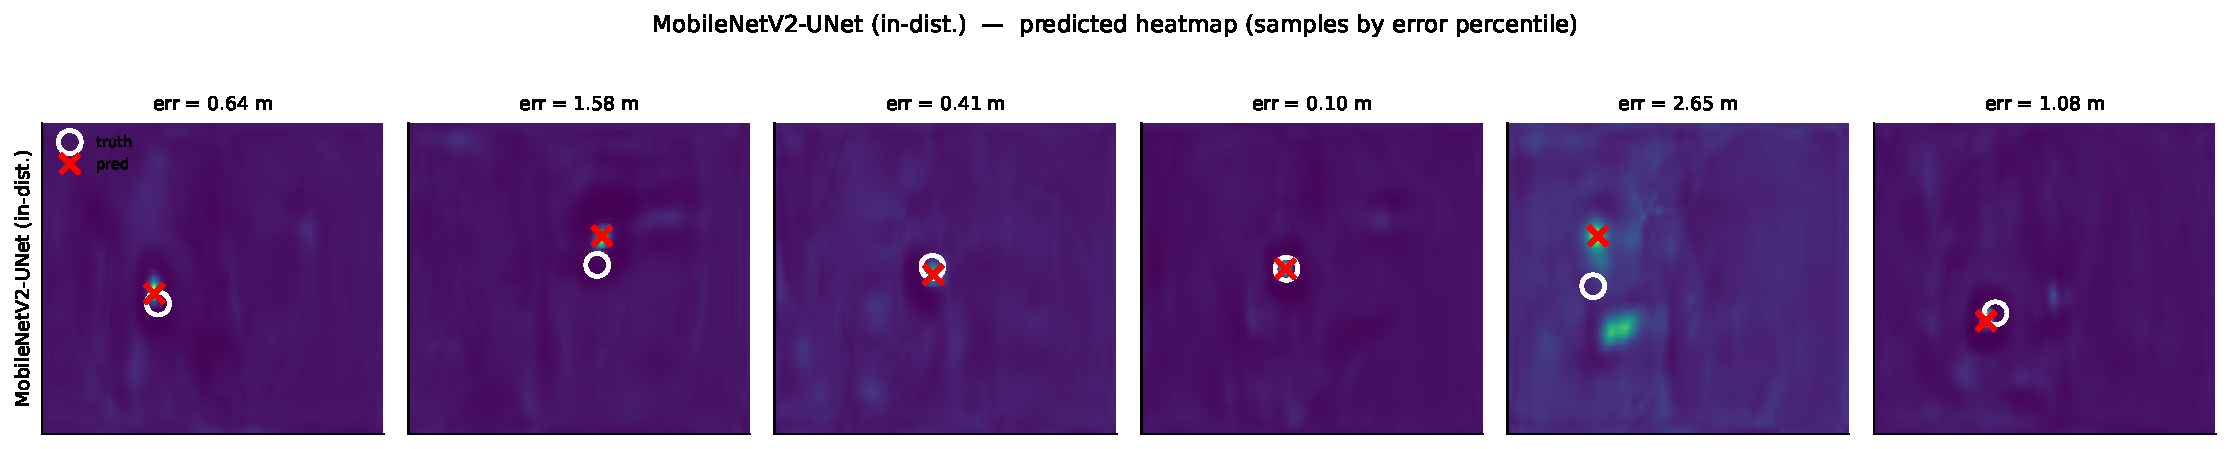
\includegraphics[width=\linewidth]{heatmaps_unet_fig10b}
\caption{Qualitative in-distribution predictions of the MobileNetV2-UNet. Each panel is a test sample
at a given error percentile; the white circle marks the ground-truth peak and the red cross the
prediction. Low-error cases (left) are tight and single-mode; the high-error case is multimodal, with
the chosen peak displaced.}
\label{fig:arch:hm_indist}
\end{figure}

\begin{whybox}
\textbf{Why it beats the teacher:} the skip connections feed the decoder the \emph{high-resolution
spatial detail} that the bottleneck throws away (Sec.~\ref{sec:blocks:unet}). Since the answer
\emph{is} a precise spatial location, restoring that detail directly lowers the error ---0.640 beats
DLoc's 0.707 with $6.8\times$ fewer parameters. \textbf{Why it is so noise-robust:} those same shallow
features travel a short path that bypasses the noise-amplifying bottleneck, so a corrupted latent no
longer dooms the prediction ($5.5\times$ better than plain MobileNetV2) ---an \emph{architectural}
robustness, independent of distillation. \textbf{Why it trails slightly on the reflector median:} it
has no consistency decoder to enforce cross-AP agreement, and that mechanism is exactly what helps most
under the aluminum reflector's strong specular multipath; the qualitative heatmaps there show extra
``phantom'' probability mass. Even so it still wins the reflector \emph{P90}, so the gap is small and
confined to the hardest fold.
\end{whybox}

\begin{figure}[H]
\centering
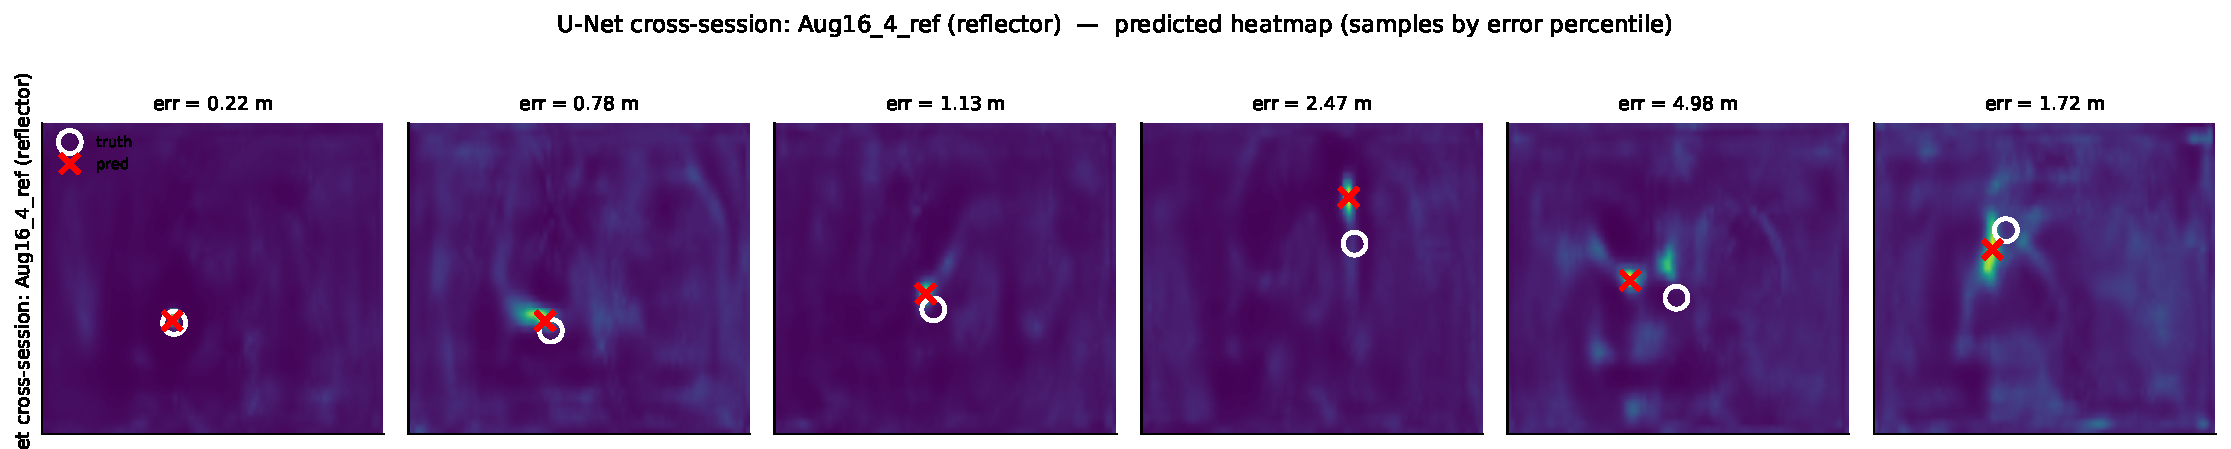
\includegraphics[width=\linewidth]{heatmaps_unet_cross_env4}
\caption{Qualitative cross-session predictions on the reflector fold (Aug16\_4\_ref). Compared with the
in-distribution panels of Figure~\ref{fig:arch:hm_indist}, the heatmaps carry extra scattered
probability mass ---the specular ``phantom'' reflections from the aluminum panel--- which drives the
larger errors on this fold and is exactly what the absent consistency decoder would suppress.}
\label{fig:arch:hm_reflector}
\end{figure}

%% ===================================================================
\section{Mamba --- the instructive negative result}
\label{sec:arch:mamba}

\begin{ataglance}{Mamba}
\textbf{Role:} a deliberately different inductive bias.\quad \textbf{Params:} 0.65\,M.\quad
\textbf{Compression:} $25\times$.\quad \textbf{Verdict:} fails to learn the task (worst median of all),
and the failure is \emph{diagnostic} ---it isolates why the image framing matters.
\end{ataglance}

\paragraph{The architecture.} A \textbf{selective state-space (Mamba) model}
(Sec.~\ref{sec:blocks:mamba}) with $\approx$0.65\,M parameters. Unlike every other model, it does
\emph{not} treat the CSI as a 2D image; it flattens each AP's measurements into a \textbf{1D sequence}
and processes them with a recurrent state.

\paragraph{Concepts it embodies.} State-space sequence modeling with a content-selective recurrence.
Its whole reason for existence is to test whether a non-convolutional, sequence-style inductive bias
can compete on the CSI-to-heatmap problem.

\paragraph{Its results.} It reaches a median of \worst{10.56\,m} (P90~$20.0$, P99~$28.3$) ---the worst
of any model, placing it at the unfavorable top of the accuracy--size plane. Tellingly, it achieves
its \emph{best} accuracy at the very first epoch and then degrades \emph{monotonically}, with training
and test error rising \emph{together}.

\begin{whybox}
\textbf{Why it fails ---and why it is \emph{not} a capacity problem:} at 0.65\,M parameters Mamba is
larger than the 47\,K TinyCNN, yet far worse, so size is not the issue. The cause is an
\textbf{architectural mismatch}. The target is an inherently 2D spatial heatmap, but an SSM consumes a
1D ordered sequence; flattening the grid imposes an arbitrary scan order that \emph{destroys spatial
locality} ---pixels that are physical neighbors land far apart in the sequence. \textbf{Why we know it
is mismatch, not overfitting:} in overfitting, training error falls while test error rises. Here both
rise together after epoch~1, so the model is not memorizing the data; the selective state-space bias
is simply ill-suited to the problem. The result is kept because a clean negative result is itself
evidence: it confirms that the image-to-image \emph{framing} (Sec.~\ref{sec:found:translation}), not
merely ``a small modern network,'' is what makes the other students work.
\end{whybox}

\section{Reading the five together}
\label{sec:arch:together}

Lined up, the five models tell one story along the size axis. DLoc shows the task is solvable but
over-provisions capacity. MobileNetV2 strips that capacity away \emph{losslessly}, proving the excess
was redundant. TinyCNN strips \emph{too} much and falls through the capacity floor. The
MobileNetV2-UNet adds back the \emph{right} thing ---skip connections, not raw parameters--- and
overtakes the teacher. Mamba changes the \emph{framing} instead of the size and breaks, isolating the
image assumption as load-bearing. Chapter~\ref{ch:findings} turns these five vertical stories into the
six horizontal findings of the thesis.
